% !TEX root = Krylov_QMC.tex
\section{Computational Results}
\label{sec:results}


 %%%%%%%%%%%%%%%%%%%%%%%%%%%%%%%%%%%%%%%%%%%%%%%%%%%%%%%%%%%%%%%%%%
 %%%%%%%%%%%%%%%%%%%%%%%%%%%%%%%%%%%%%%%%%%%%%%%%%%%%%%%%%%%%%%%%%%
\subsection{Garcia-Siewert}

The first computations use the problem from Garcia et al. \cite{cesinh}, outlined in Table ~\ref{tab:garcia}, and consider two cases for the scattering cross section ($\Sigma_s = e^{-x/s}$), $s=1$ and $s=\infty$. First, we solve the QMC linear problem with $N=2048$ and $N_x=100$.  Figure ~\ref{fig:easy} shows that for an exponentially decaying scattering cross section ($s=1$) the Krylov iterations take fewer than a third of the number of transport sweeps than that of the Picard iteration for a relative residual of $10^{-9}$. While Figure ~\ref{fig:hard} ($s=\infty$) shows the Krylov iterations took less than 25 iterations to reach a relative error of $10^{-6}$ while the Picard iteration required nearly 200 iterations. 

\begin{table}[h]
\centering
\caption{Parameters for fixed boundary source, slab geometry, simulation from Garcia et al. \cite{cesinh}}
\label{tab:garcia}
\centerline{
\begin{tabular}{c | c}
\hline
 Parameter & Value \\ 
\hline
 $\Sigma_t$ & 1 \\  
 $\Sigma_s(x)$ & $e^{-x/s}$ \\
 $\tau$ & $5$ \\
 $\psi_l(\mu)$ & 1 \\
 $ \psi_r(\mu)$ & 0 \\
 $N_x$ & 50 \\
 $q(x)$ & 0 \\
\hline
\end{tabular}
}
\end{table}

%\vspace*{.25in}

\begin{figure}[h]
\centerline{
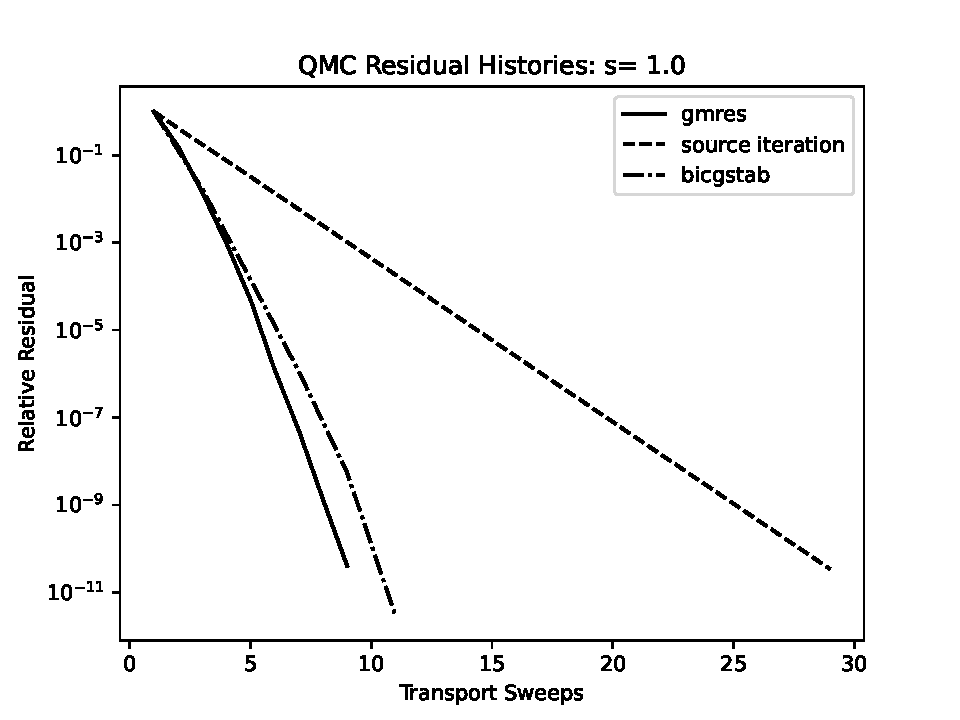
\includegraphics[width=3.5in]{FIGURES/seqone.pdf}
}
\caption{\label{fig:easy} Scalar flux relative residuals for $s=1$ given parameters from Table ~\ref{tab:garcia} and $N=2048$.}
\end{figure}

\begin{figure}[h]
\centerline{
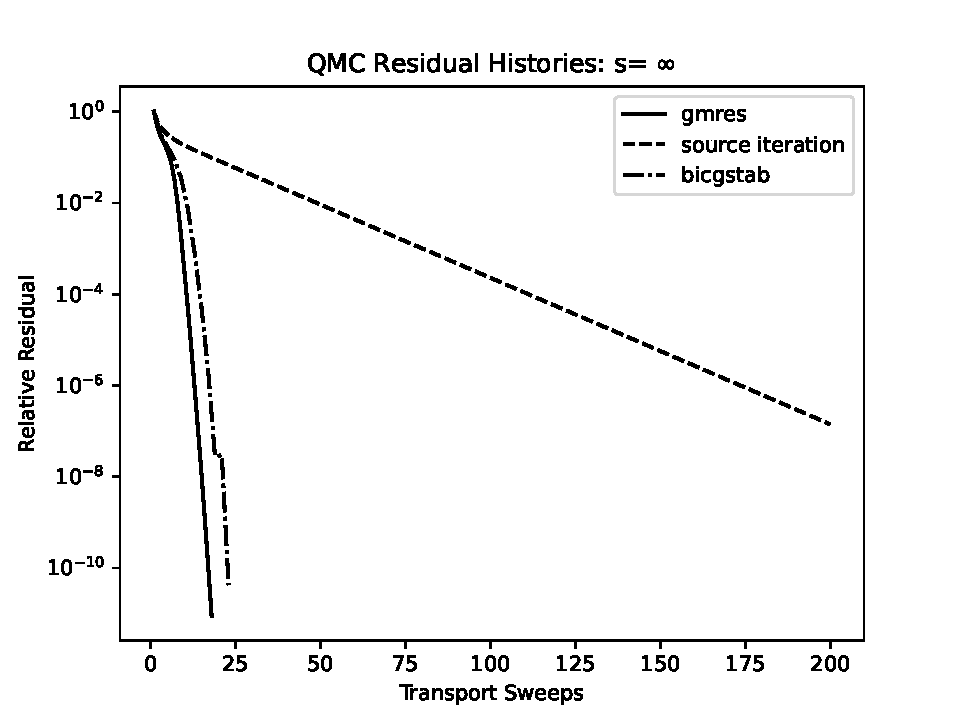
\includegraphics[width=3.5in]{FIGURES/seqinf.pdf}
}
\caption{\label{fig:hard} Scalar flux relative residuals for $s=\infty$ given parameters from Table ~\ref{tab:garcia} and $N=2048$.}
\end{figure}


 %%%%%%%%%%%%%%%%%%%%%%%%%%%%%%%%%%%%%%%%%%%%%%%%%%%%%%%%%%%%%%%%%%
 %%%%%%%%%%%%%%%%%%%%%%%%%%%%%%%%%%%%%%%%%%%%%%%%%%%%%%%%%%%%%%%%%%
 
\subsubsection{Validation and calibration study}
\label{validation-and-calibration-study}

We conclude this problem with a validation study. We compare the QMC results with the results from \cite{cesinh}. The results in \cite{cesinh} are exit distributions and are accurate to six figures. We have duplicated those results with an $S_N$ computation on a fine angular and spatial mesh.

For $N=2048$ and $Nx=100$ we obtain the cell-average fluxes from the QMC approximation. We then use a single $S_N$ transport sweep to recover the exit distributions from the QMC cell-average fluxes. We report the results and the corresponding results from \cite{cesinh} in Tables~\ref{tab:cesone} and \ref{tab:cesinf}. The exit distributions, as is clear from Table~\ref{tab:cesone} can vary by five orders of magnitude. Even so, the results from QMC agree with the benchmarks to roughly two figures.

\begin{table}[h]
\centering
\caption{Angular flux exit Distributions from Garcia/Siewart and the $S_N$ QMC sweep (with $N=2048$ and $Nx=100$), along with  difference between results for $s = 1$.}
\label{tab:cesone}
\centerline{
\begin{tabular}{c | c c | c c | c c}
 & \multicolumn{2}{c}{Garcia/Siewert}
 & \multicolumn{2}{c}{QMC}
 & \multicolumn{2}{c}{Difference} \\
\hline
$\mu$ & $\psi(0, -\mu)$ & $\psi(\tau, \mu)$ & $\psi(0, -\mu)$ & $\psi(\tau, \mu)$ & $\psi(0, -\mu)$ & $\psi(\tau, \mu)$ \\
\hline
 0.05 &    5.89664e-01 &    6.07488e-06 &    6.07035e-01 &    5.91908e-06   & test & test \\ 
 0.10 &    5.31120e-01 &    6.92516e-06 &    5.47466e-01 &    6.74075e-06   & test & test \\  
 0.20 &    4.43280e-01 &    9.64232e-06 &    4.57064e-01 &    9.35453e-06   & test & test \\ 
 0.30 &    3.80306e-01 &    1.62339e-05 &    3.92223e-01 &    1.56108e-05   & test & test \\ 
 0.40 &    3.32964e-01 &    4.38580e-05 &    3.43481e-01 &    4.13721e-05   & test & test \\ 
 0.50 &    2.96090e-01 &    1.69372e-04 &    3.05510e-01 &    1.58622e-04   & test & test \\ 
 0.60 &    2.66563e-01 &    5.73465e-04 &    2.75098e-01 &    5.39514e-04   & test & test \\ 
 0.70 &    2.42390e-01 &    1.51282e-03 &    2.50192e-01 &    1.43257e-03   & test & test \\ 
 0.80 &    2.22235e-01 &    3.24369e-03 &    2.29422e-01 &    3.08975e-03   & test & test \\ 
 0.90 &    2.05174e-01 &    5.96036e-03 &    2.11837e-01 &    5.70555e-03   & test & test \\ 
 1.00 &    1.90546e-01 &    9.77123e-03 &    1.96756e-01 &    9.39189e-03   & test & test \\ 
\hline
\end{tabular}
}
\end{table}


\begin{table}[h]
\centering
\caption{Angular flux exit Distributions for: $N=2048$, $Nx=100$, and $s = \infty$.}
\label{tab:cesinf}
\begin{tabular}{lllll}
 & \multicolumn{2}{c}{Garcia/Siewert}
 & \multicolumn{2}{c}{QMC}\\
\hline
$\mu$ &$\psi(0, -\mu)$ &$\psi(\tau, \mu)$ &$\psi(0, -\mu)$ &$\psi(\tau, \mu)$ \\
\hline
0.05 &    8.97798e-01 &    1.02202e-01 &    9.06050e-01 &    1.03680e-01   \\ 
 0.10 &    8.87836e-01 &    1.12164e-01 &    8.95849e-01 &    1.13695e-01   \\ 
 0.20 &    8.69581e-01 &    1.30419e-01 &    8.76487e-01 &    1.31907e-01   \\ 
 0.30 &    8.52299e-01 &    1.47701e-01 &    8.58937e-01 &    1.49245e-01   \\ 
 0.40 &    8.35503e-01 &    1.64497e-01 &    8.42195e-01 &    1.66128e-01   \\ 
 0.50 &    8.18996e-01 &    1.81004e-01 &    8.25870e-01 &    1.82734e-01   \\ 
 0.60 &    8.02676e-01 &    1.97324e-01 &    8.09780e-01 &    1.99151e-01   \\ 
 0.70 &    7.86493e-01 &    2.13507e-01 &    7.93834e-01 &    2.15421e-01   \\ 
 0.80 &    7.70429e-01 &    2.29571e-01 &    7.77997e-01 &    2.31558e-01   \\ 
 0.90 &    7.54496e-01 &    2.45504e-01 &    7.62269e-01 &    2.47547e-01   \\ 
 1.00 &    7.38721e-01 &    2.61279e-01 &    7.46673e-01 &    2.63362e-01   \\ 
\hline
\end{tabular}
\end{table}

In Tables \ref{tab:bigtab1} and \ref{tab:bigtabinf} we look at the relative errors in the QMC exit distributions as compared to a highly accurate $S_N$ result. We compensate for the widely varying scales by tabulating, for each value of $N$ and $Nx$
\[
R = \max(R^0, R^\tau)
\]
where
\[
R^0 = \max_\mu
\frac{ | \psi^{SN}(0,-\mu) - \psi^{QMC}(0,-\mu) | }{\psi^{SN}(0,-\mu) }
\]
and
\[
R^\tau = \max_\mu
\frac{ | \psi^{SN}(\tau,\mu) - \psi^{QMC}(\tau,\mu) | }{\psi^{SN}(\tau,\mu) }.
\]

\begin{table}[h]
\centering
\caption{Exit Distributions Errors: $s = 1.0$}
\label{tab:bigtab1}
\begin{tabular}{l|lllll} 
\hline
 Nx \textbackslash N &     1024 &     2048 &     4096 &     8192 &    16384 \\ 
\hline 
50 & 1.31716e-01& 1.34260e-01& 1.35123e-01& 1.35328e-01& 1.35242e-01   \\ 
100 & 6.09631e-02& 6.35764e-02& 6.46191e-02& 6.48898e-02& 6.48536e-02   \\ 
200 & 3.77223e-02& 3.12496e-02& 3.12005e-02& 3.17337e-02& 3.16710e-02   \\ 
400 & 2.63214e-02& 1.45106e-02& 1.52355e-02& 1.56636e-02& 1.56854e-02   \\ 
800 & 2.39486e-02& 9.94925e-03& 7.24627e-03& 8.86212e-03& 7.84063e-03   \\ 
1600 & 4.16277e-02& 9.95048e-03& 5.11618e-03& 8.02709e-03& 4.44021e-03   \\ 
3200 & 4.60905e-02& 1.07345e-02& 4.45922e-03& 7.49522e-03& 3.76179e-03   \\ 
\hline 
\end{tabular} 
\end{table}

\begin{table}[h]
\centering
\caption{Exit Distributions Errors: $s = \infty$}
\label{tab:bigtabinf}
\begin{tabular}{l|lllll} 
\hline
 Nx \textbackslash N &     1024 &     2048 &     4096 &     8192 &    16384 \\ 
\hline 
50 & 1.31716e-01& 1.34260e-01& 1.35123e-01& 1.35328e-01& 1.35242e-01   \\ 
100 & 6.09631e-02& 6.35764e-02& 6.46191e-02& 6.48898e-02& 6.48536e-02   \\ 
200 & 3.77223e-02& 3.12496e-02& 3.12005e-02& 3.17337e-02& 3.16710e-02   \\ 
400 & 2.63214e-02& 1.45106e-02& 1.52355e-02& 1.56636e-02& 1.56854e-02   \\ 
800 & 2.39486e-02& 9.94925e-03& 7.24627e-03& 8.86212e-03& 7.84063e-03   \\ 
1600 & 4.16277e-02& 9.95048e-03& 5.11618e-03& 8.02709e-03& 4.44021e-03   \\ 
3200 & 4.60905e-02& 1.07345e-02& 4.45922e-03& 7.49522e-03& 3.76179e-03   \\ 
\hline 
\end{tabular} 
\end{table}


%%%%%%%%%%%%%%%%%%%%%%%%%%%%%%%%%%%%%%%%%%%%%%%%%%%%%%%%%%%%%%%%%%
 %%%%%%%%%%%%%%%%%%%%%%%%%%%%%%%%%%%%%%%%%%%%%%%%%%%%%%%%%%%%%%%%%%

\subsection{Multigroup Problems}

The second problem features 12, 70, and 618 group cross section data of high-density polyethylene generated with FUDGE \cite{mattoon2012generalized} in an infinite medium.  The analytic solution of the scalar flux is given by:
\begin{equation}
    \phi = (\Sigma_t - \Sigma_s)^{-1}Q.
\end{equation}

These are preliminary results with $N_x = 40$ and $N=2^{10}$. We may want to make these larger and/or make tables like  Table~\ref{tab:bigtab1} and Table~\ref{tab:bigtab1}. 


\begin{figure}
     \centering
     \begin{subfigure}[b]{0.45\textwidth}
         \centering
         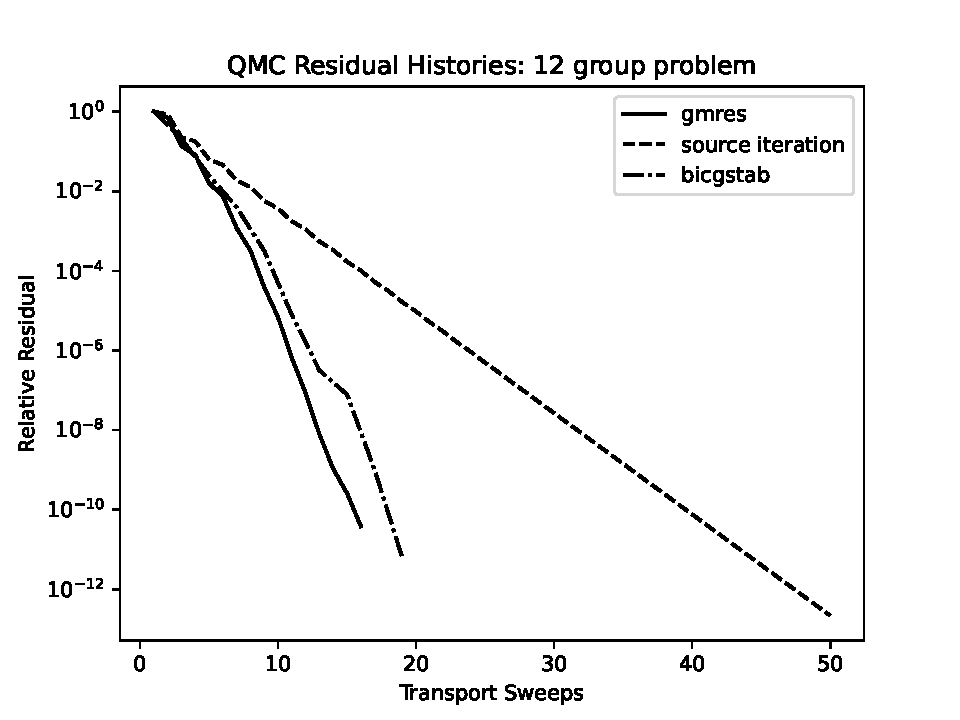
\includegraphics[width=\textwidth]{FIGURES/12Group.pdf}
         \caption{\label{fig:618group}}
     \end{subfigure}
     \hfill
     \begin{subfigure}[b]{0.45\textwidth}
         \centering
         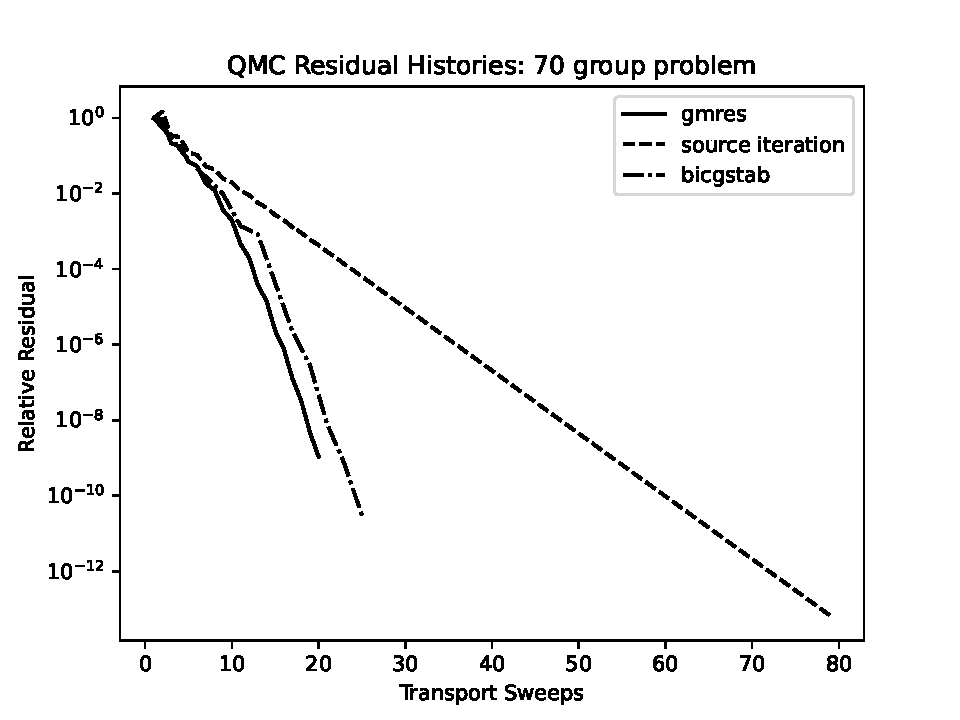
\includegraphics[width=\textwidth]{FIGURES/70Group.pdf}
         \caption{\label{fig:70group}}
     \end{subfigure}
     \\
     \begin{subfigure}[b]{0.45\textwidth}
         \centering
         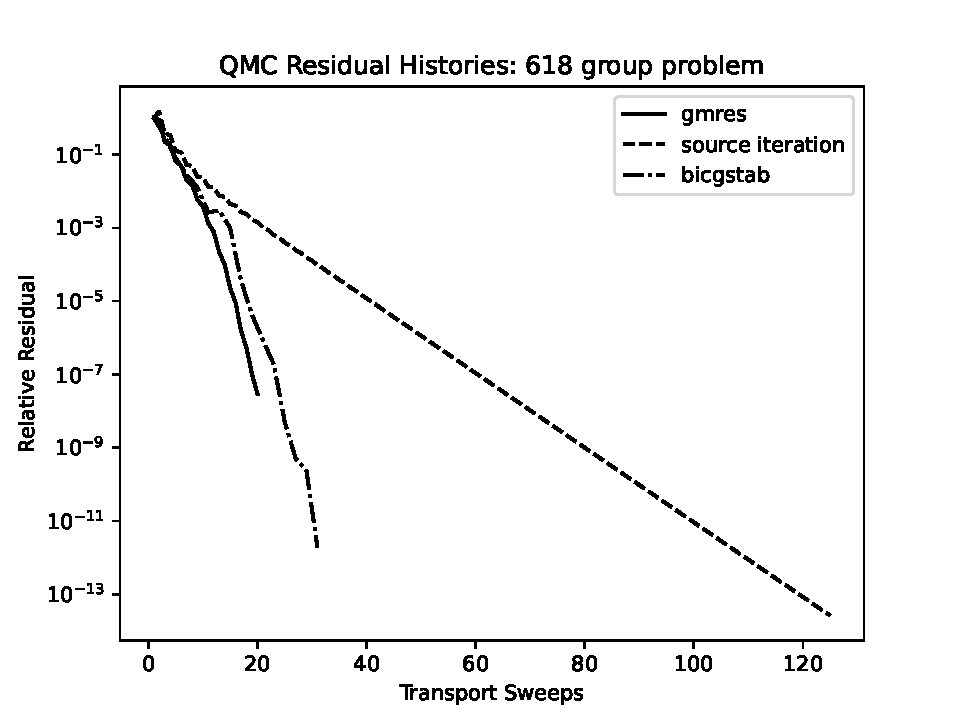
\includegraphics[width=\textwidth]{FIGURES/618Group.pdf}
         \caption{\label{fig:12group}}
     \end{subfigure}
        \caption{Multigroup relative residuals defined as $||\phi_n - \phi_{n-1}||$ for 12, 70, and 618 group problems.}
        \label{fig:multigroup}
\end{figure}

%%%%%%%%%%%%%%%%%%%%%%%%%%%%%%%%%%%%%%%%%%%%%%%%%%%%%%%%%%%%%%%%%%
 %%%%%%%%%%%%%%%%%%%%%%%%%%%%%%%%%%%%%%%%%%%%%%%%%%%%%%%%%%%%%%%%%%

\subsection{Reed's Problem}

\begin{figure}[h]
\centerline{
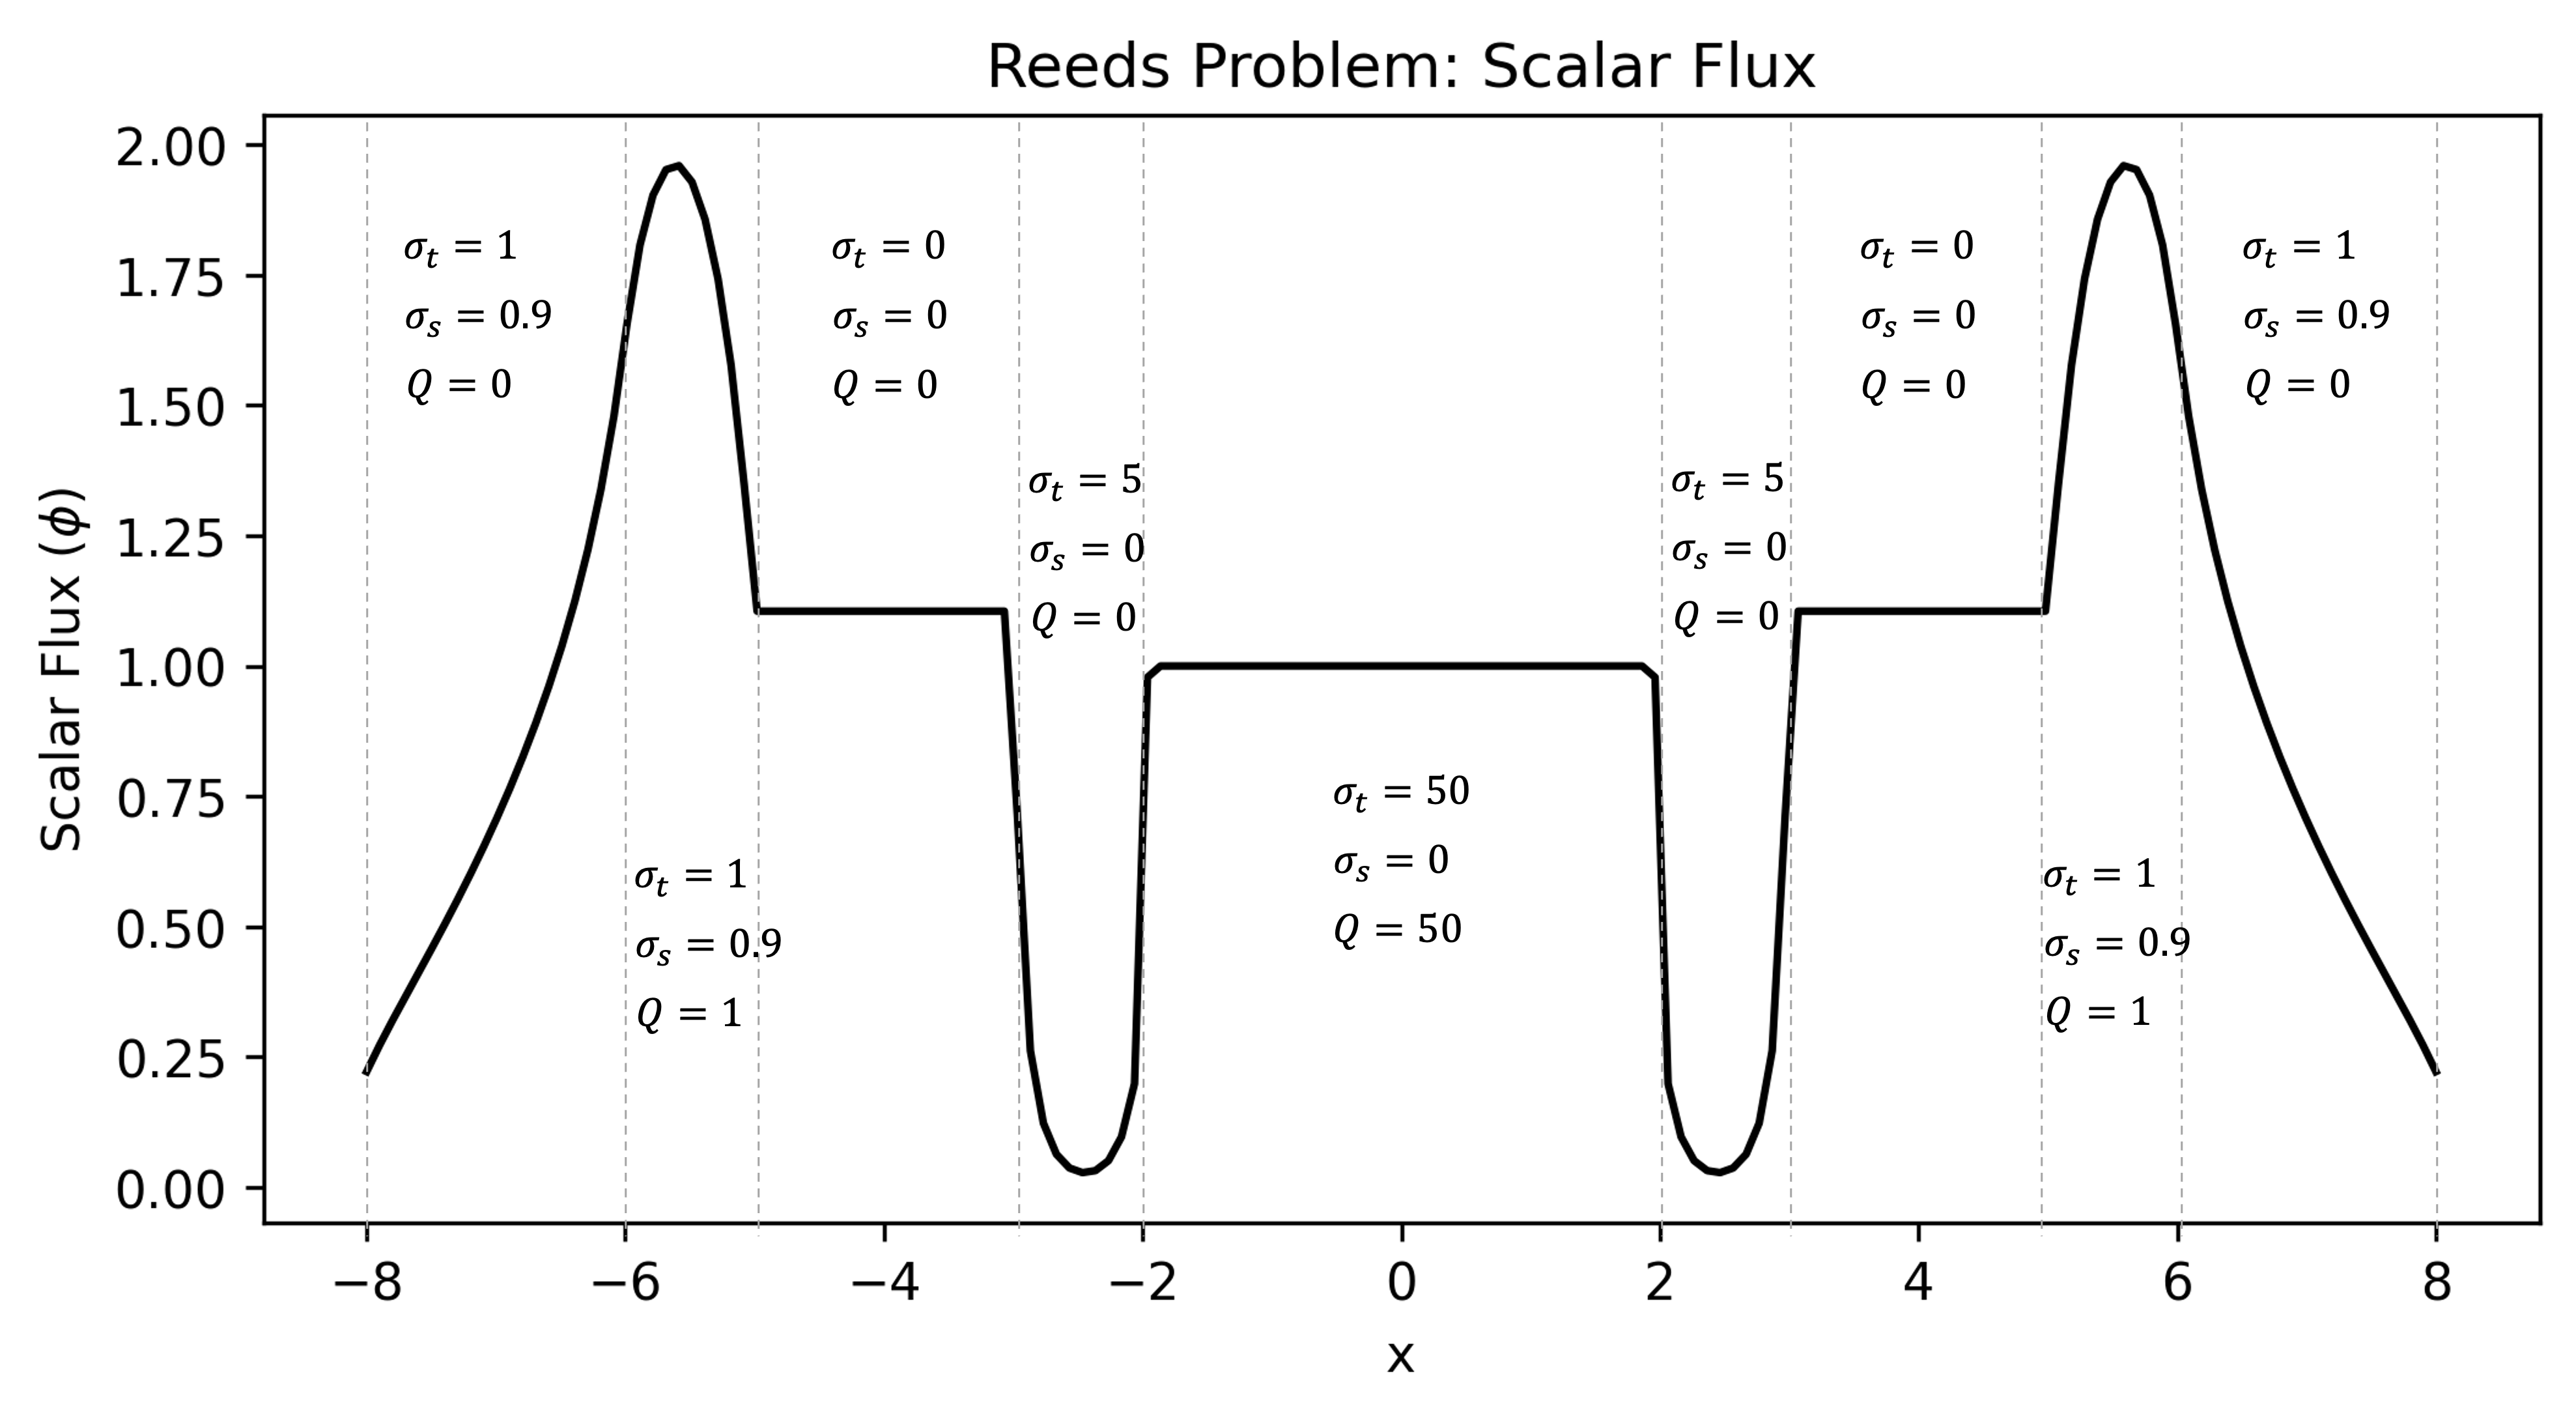
\includegraphics[width=5.5in]{FIGURES/Reeds_problem2.png}
}
\caption{\label{fig:reeds}}
\end{figure}

\begin{figure}[h]
\centerline{
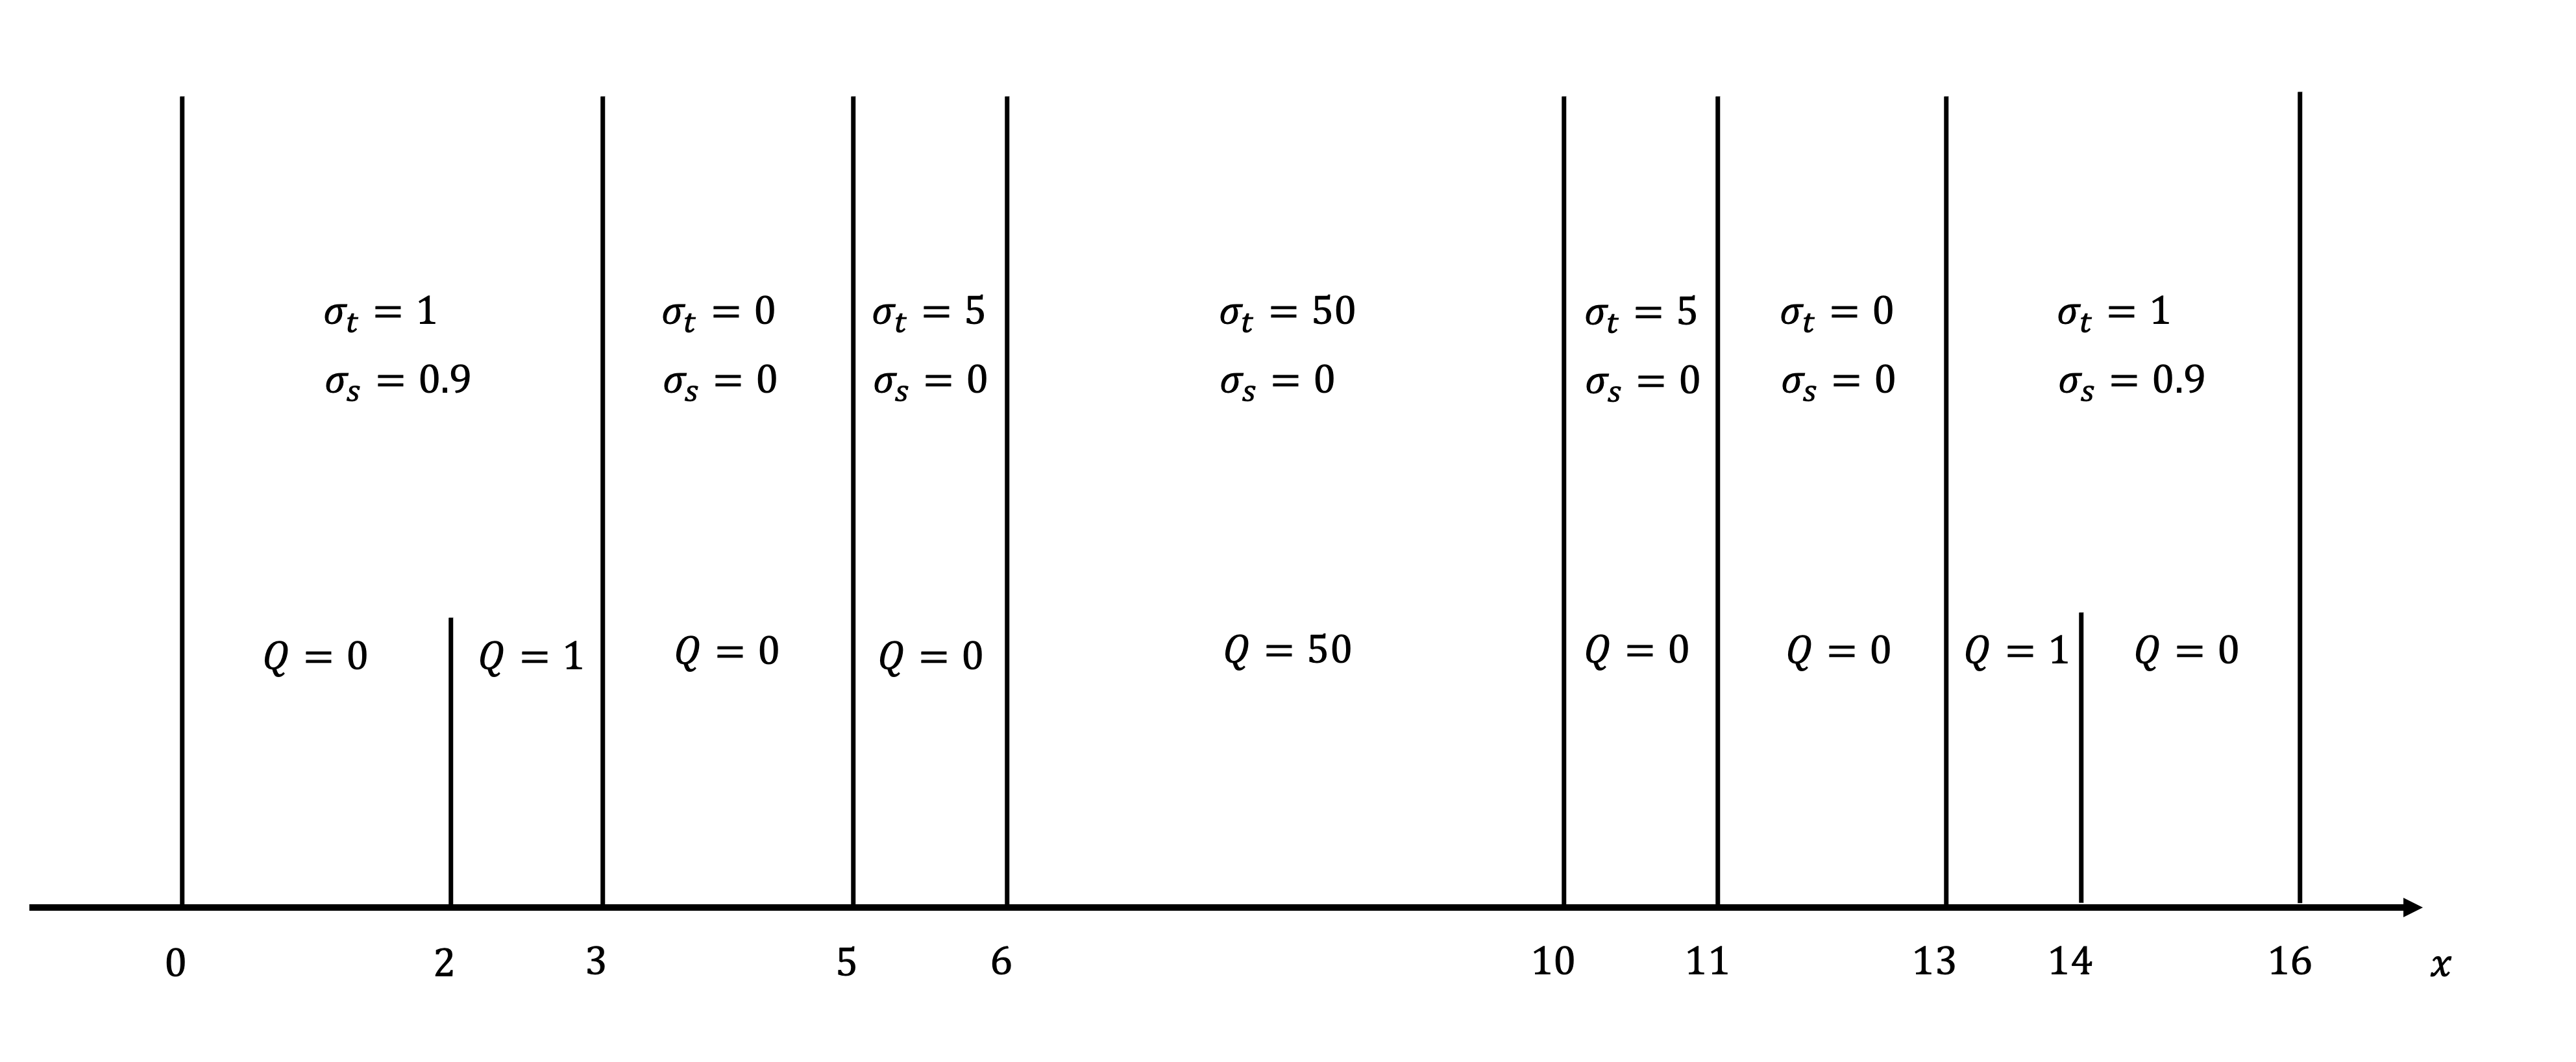
\includegraphics[width=5.0in]{FIGURES/Reeds_problem.png}
}
\caption{\label{fig:reeds}}
\end{figure}